\documentclass{article}
\usepackage{tikz}

\begin{document}

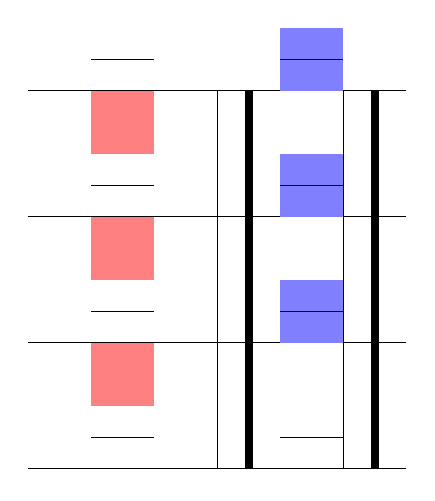
\begin{tikzpicture}[scale=0.8]
    % Draw horizontal lines
    \draw (0,0) -- (6,0);
    \draw (0,2) -- (6,2);
    \draw (0,4) -- (6,4);
    \draw (0,6) -- (6,6);
    
    % Draw vertical lines
    \draw (3,0) -- (3,6);
    \draw (5,0) -- (5,6);
    
    % Draw red rectangles
    \fill[red!50] (1,1) rectangle (2,2);
    \fill[red!50] (1,3) rectangle (2,4);
    \fill[red!50] (1,5) rectangle (2,6);
    
    % Draw blue rectangles
    \fill[blue!50] (4,2) rectangle (5,3);
    \fill[blue!50] (4,4) rectangle (5,5);
    \fill[blue!50] (4,6) rectangle (5,7);
    
    % Draw black vertical line
    \draw[line width=1mm] (3.5,0) -- (3.5,6);
    \draw[line width=1mm] (5.5,0) -- (5.5,6);
    
    % Draw horizontal line above blue rectangles
    \draw (4,0.5) -- (5,0.5);
    \draw (4,2.5) -- (5,2.5);
    \draw (4,4.5) -- (5,4.5);
    \draw (4,6.5) -- (5,6.5);
    
    % Draw horizontal line below blue rectangles
    \draw (4,0.5) -- (5,0.5);
    \draw (4,2.5) -- (5,2.5);
    \draw (4,4.5) -- (5,4.5);
    \draw (4,6.5) -- (5,6.5);
    
    % Draw horizontal line above red rectangles
    \draw (1,0.5) -- (2,0.5);
    \draw (1,2.5) -- (2,2.5);
    \draw (1,4.5) -- (2,4.5);
    \draw (1,6.5) -- (2,6.5);
    
    % Draw horizontal line below red rectangles
    \draw (1,0.5) -- (2,0.5);
    \draw (1,2.5) -- (2,2.5);
    \draw (1,4.5) -- (2,4.5);
    \draw (1,6.5) -- (2,6.5);
\end{tikzpicture}

\end{document}